\documentclass[10pt,a4paper]{article}

\usepackage[utf8x]{inputenc}
\usepackage[english]{babel}
\usepackage[T1]{fontenc,url}
\usepackage[hang,small,bf]{caption}
\usepackage{relsize}
\usepackage{setspace}
\usepackage{parskip}
\usepackage{lmodern}
\usepackage{microtype}
\usepackage{verbatim}
\usepackage{amsmath, amssymb, amsthm}
\usepackage{mathtools}
\usepackage{tikz}
\usepackage{physics}
\usepackage{algorithm}
\usepackage{algpseudocode}
\usepackage{listings}
\usepackage{enumerate}
\usepackage{graphicx}
\usepackage{float}
\usepackage[hidelinks]{hyperref}
\usepackage{varioref}
\usepackage{siunitx}
\usepackage{todonotes}
\usepackage{color}
\usepackage[margin=3cm]{geometry}
\labelformat{equation}{equation~(#1)}

\renewcommand{\exp}{\mathrm{e}^}
\newcommand{\halflife}{t_{\frac{1}{2}}}
\newcommand{\half}{\frac{1}{2}}
\newcommand{\planck}{$h = \SI{6.626e-34}{J.s}$}

\definecolor{light_green}{rgb}{0, 0.6, 0}
\definecolor{light_grey}{rgb}{0.5, 0.5, 0.5}
\definecolor{magenta}{rgb}{0.7, 0, 0.5}


\lstdefinestyle{py}{
    language = python,
    frame = single,
    showstringspaces = false,
    basicstyle = \small\ttfamily,
    breaklines = true,
    commentstyle = \color{light_grey},
    keywordstyle = \color{magenta},
    stringstyle = \color{light_green},
}


\begin{document}

\section*{Exercise 5.1 - Pulling crates}
\addcontentsline{toc}{section}{Exercise 5.1 - Pulling crates - \texttt{pull\_crates.py}}

We will look at the case where $N$ connected crates are being pulled by someone:
\begin{center}
	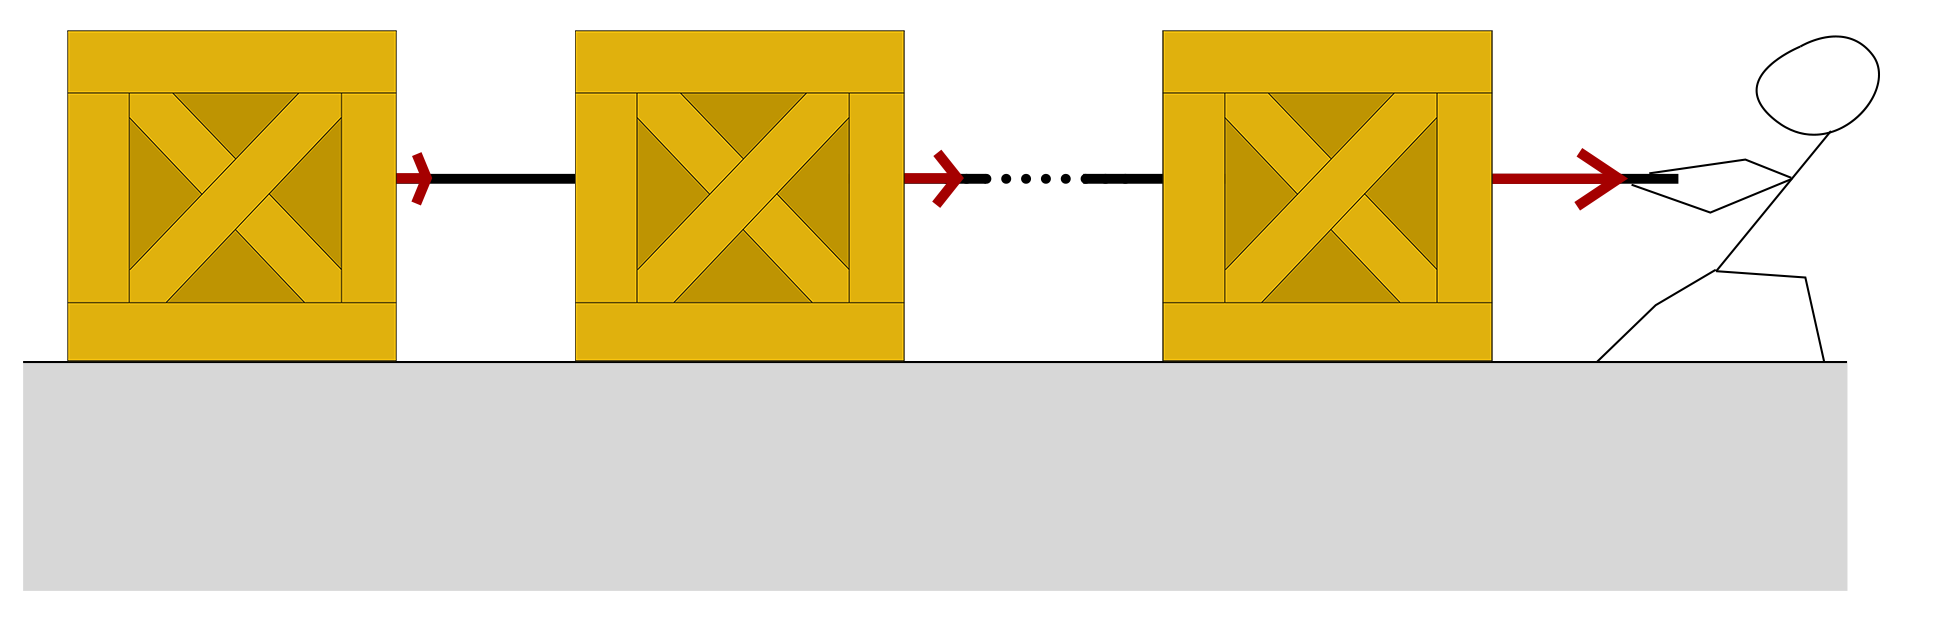
\includegraphics[scale=1]{fig_pull_crates-cp1.png}\\
	\captionof{figure}{Illustration of a person pulling some creates. The dots indicates that there are arbitrary number of crates and the red arrows the direction and strength of the force exterted on the crates.}
\end{center}

\subsection*{a)}
We have measured that every $i$-th create is influenced by a force of $30 + 5\cdot i\,\si{\newton}$. 

Write a program which generates a list of the forces which acts on every $i$-th create. Here we will look at $N = 10$ crates. 

\subsection*{b)}
It turns out that the forces measured in a), turned out to be too large. Divide the values form a) by 2 \textit{without} using for or while loops. Find the sum of the values, also without for or while loops, and then print the result. 


Filename: \texttt{pull\_crates.py}



\section*{Exercise 5.2 - Plotting relativistic against classical momentum}
\addcontentsline{toc}{section}{Exercise 5.2 - Plotting relativistic against classical momentum - \texttt{momentum\_plot.py}}
The momentum of an object with mass $m$ and velocity $v$ is defined differently in classical and relativistic physics:
\begin{align*}
p_{clas} &= m\cdot v
\\
p_{rel} &= m\cdot v\cdot \gamma, \ \ \ \ \gamma = \frac{1}{\sqrt{1-\frac{v^2}{c^2}}}
\end{align*}
The speed of light is defined as $c \approx \SI{3e8}{m/s}$.

Set $m = \SI{5}{kg}$, and plot the two functions in the same plot, with velocities evenly distributed in the interval $v \in [0c,\ 0.9c] = [\SI{0}{m/s},\ \SI{2.7e8}{m/s}]$.

Filename: \texttt{momentum\_plot.py}


\section*{Exercise 5.3 - capacitor discharge}
\addcontentsline{toc}{section}{Exercise 5.3 - capacitor discharge - \texttt{capacitor\_vectorization.py}}
\textbf{Physical introduction:} A capacitor is simply two metal plates set up parallell to each other. We can charge up each plate with positive and negative electic charges by connecting them to a battery. If we remove the battery and connect the two plates together, the charges will flow from the negative plate to the positive plate, and the capacitor will discharge. To avoid the electrical current becoming infinite, we connect a resistor between the plates. We now have an RC-circuit.

The charge $Q$ of a capacitor that discharges in a RC-circuit, is given as
\begin{align*}
Q(t) = CV\exp{-t/RC}
\end{align*}

The following program calculates this discharge for $n=1000$ time-steps over an interval $t = \SI{10}{s}$. The capacitor has a \textit{capacitance} of $C = \SI{0.007}{F}$, an initial voltage $V_0 = \SI{50}{V}$, and the resistor has a resistance $R = \SI{350}{\ohm}$.

\lstinputlisting[style=py]{capacitor.py}

Copy the program and confirm that it works as intended.

Vectorize the program such that \texttt{t\_list} and \texttt{I\_list} is replaced by numpy vectors, and the for loops are replaced by vector operations. Confirm that the result remains the same.

Filename: \texttt{capacitor\_vectorization.py}


\section*{Exercise 5.4 - Planck's Law}
\addcontentsline{toc}{section}{Exercise 5.4 - Planck's Law - \texttt{Planck\_curves.py}}

Planck's law describes how much energy a black body (usually a star) emmits at different wavelengths of electromagnetic radiation. The law is given as
\begin{align*}
B(\lambda) = \frac{2hc^2}{\lambda^5}\frac{1}{\exp{\frac{hc}{\lambda k T}}-1}
\end{align*}
where $T$ is the temperature of the star, $h = \SI{6.62e-34}{J.s}$ is Planck's constant, $k = \SI{1.38e-23}{J/K}$ is Boltzmanns constant, and the speed of light is still $c \approx \SI{3e8}{m/s}$. The plots that comes from plotting this function are called 'Planck curves', and is a common sight in physics books.


\subsection*{a)}
Use the temperature of the sun, $T = \SI{5800}{K}$, and plot $B(\lambda)$ against wavelengths in the interval $\lambda \in [\SI{10}{nm},\ \SI{3000}{nm}]$. Note that these wavelengths are in nanometers, while the function takes wavelengths in meters.


\subsection*{b)}
Include also the Planck curves of the stars Alpha Centauri A ($T = \SI{25 000}{K}$), and Proxima Centauri ($T = \SI{2400}{K}$), in the same plot as the Sun.

\subsection*{c)}
Wien's displacement law tells us that we should find the peak of the Planck curve at the wavelength
\begin{align*}
\lambda_{max} = \frac{b}{T}
\end{align*}
where $b = 2.9\cdot 10^{-3}\,\mathrm{Km}$ is called Wien's displacement constant.

Expand the plot from b) by adding three vertical lines at $x = \lambda_{max}$ for each of the three stars, and confirm that the lines corresponds to the peak of the curves.

\textbf{Hint}: You can make vertical lines in Python with the function \texttt{matplotlib.pyplot.axvline(x= )}

Filename: \texttt{Planck\_curves.py}




\section*{Exercise 5.5 - Oscilating spring}
\addcontentsline{toc}{section}{Exercise 5.5 - Oscilating spring - \texttt{oscilating\_spring.py}}
A rock of mass $m$ is hung from a spring, and dragged down a length $A$. Upon release, the rock will oscilate up and down with a vertical position given as
\[	y(t) = A\cdot \exp{-\gamma t}\cos\left(\sqrt{\frac{k}{m}}\cdot t\right)
\]
Here, $y=0$ corresponds to the vertical position of the rock when just hanging still from the spring. Set $k = \SI{4}{kg/s^2}$ and $\gamma = \SI{0.15}{s^{-1}}$. Assume the rock has a mass $m = \SI{9}{kg}$, and that you drag the rock down a length $A = \SI{0.3}{m}$.

\subsection*{a)}
Create empty arrays \texttt{t\_array} and \texttt{y\_array} of size 101. Use a for loop to fill them with time values in the range $[\SI{0}{s},\ \SI{25}{s}]$, and the corresponding $y(t)$ values.

\subsection*{b)}
Vectorize your program by instead using the \texttt{linspace} function to generate the array \texttt{t\_array}, and send it into a function \texttt{y(t)} to genereate the array \texttt{y\_array}. Your program should now be free of for loops.

\subsection*{c)}
Plot the position of the rock against time in the given time interval. Use the arrays from both exercise a) and b), and confirm that they give the same result. Get correct units on each axis.

Filename: \texttt{oscilating\_spring.py}






\section*{Exercise 5.6 - Planatary motion}
\addcontentsline{toc}{section}{Exercise 5.6 - Planatary motion - \texttt{planetary\_motion.py}}

The motion of a planet orbiting a star can be described by its distance to its star as a function of its anglular position:
\begin{equation}
r(\theta) = \frac{p}{1+e\cos(\theta)}	\label{eqn:radial_orbit}
\end{equation}
where
\begin{itemize}
\item $\theta$ simply represents where in its orbit the planet is (in radians). $\theta = 0$ is angle where the planet is closest to it's star.

\item $p$ is just a parameter representing the size of the orbit, which we will set to 1 AU. \footnote{This is the average distance from our sun to the earth. We will use it as our distance-unit in all plots and calculations.}

\item $e$ is the \textit{eccentrisity} of the orbit, which says how eliptical the orbit is. $e = 0$ represents a circular orbit, and $e\geq 1$ means that the planet is not even in an orbit around the star, and simply traveling by.
\end{itemize}


\subsection*{a)}
Plot the planet's distance to the star as a function of angular position for eccentrities $e = 0$, $e = 0.5$, and $e = 0.8$ in the same plot. Use $\theta \in [0,\ 2\pi]$ to include one full orbit of the planet. Get correct units on both axis.


\subsection*{b)}
You shall now plot the actual orbits of the planet, for each of the three eccentrities. To make the plotting easier, we decompose \ref{eqn:radial_orbit} into x and y coordinates:
\[	x(\theta) = r(\theta)\sin(\theta),\ \ \ \ y(\theta) = r(\theta)\cos(\theta)
\]

Use these equations to plot $y(\theta)$ against $x(\theta)$, still using $\theta \in [0,\ 2\pi]$, for each of the three eccentrities.

Remember that both $r(\theta)$ and $\theta$ are arrays, and the resulting $x(\theta)$ and $y(\theta)$ are also arrays, and can simply be plotted against each other as they are.

\textbf{Hint:} Matplotlib doesn't keep axis proportional by default, meaning that a circular motion might look elliptical on the plot. If you include the line \texttt{matplotlib.pyplot.axis('equal')}, the x and y coordinates will be of equal scale.
You can also include the star itself, to make the plot more visually appealing. Do this by plotting a point at (0,0), and specify it as a yellow dot: \texttt{matplotlib.pyplot.plot(0, 0, 'yo')}

Filename: \texttt{planetary\_motion.py}



\section*{Exercise 5.7 - Estimate the value of Planck's constant}
\addcontentsline{toc}{section}{Exercise 5.7 - Estimate the value of Planck's constant - \texttt{estimate\_h.py}}

It is possible to use some data points to estimate the value of Planck's constant $h$. To do so, we will use Einstein's equation describing the photoelectric effect\footnote{The equation came to life when Einstein wanted to explain why the photoelectric effect occurs, i.e why electrons can set free from metal if the light as a high enough frequency.}. 

The equation found by Einstein is:
\begin{align*}
	E_k = hf - W 
\end{align*} 
where $h$ is Planck's constant, $f$ is the frequency of the light, $W$ is the work which is needed to free the electrons and $E_k$ is the electrons maximum kinetic energy.  

Suppose we have gotten some measurements from one experiment where we have sent light with different frequencies $f$ such that the electrons got a maximum kinetic energy $E_{k,max}$:
\begin{center}
\begin{tabular}{l|c|c|c|c}
	$f/10^{15}\,$Hz & 1.18 & 0.96 & 0.82 & 0.74 \\ \hline 
	$E_{k,max}/10^{-19}\,\mathrm{J}$ & 3.12 & 1.57 & 0.8 &  0.22
\end{tabular} 
\end{center}
The frequencies of light $f$ in the table has been divided by $10^{15}$. Similar goes for the maximum kinetic energies $E_k$ in the table where the values haven been divided by  $10^{-19}$. Remember, when you have to use these values it is necessary to multiply the values of $f$ and $E_{k,max}$ by   $10^{15}$ and $10^{-19}$ respectively!

\subsection*{a)}
Write a program which plots the measurements as points. The values for $f$ and $E_{k,max}$ should be in arrays. Plot the values for $f$ along the x-axis and the values for $E_{k,max}$  along the y-axis. 

\textbf{Hint:} To plot the points, it is enough to send an additional parameter to \texttt{plt.plot} to indicate that you want to plot points instead of lines. For instance, if you want red points, you could send \texttt{'ro'} as the additional parameter to \texttt{plt.plot}.

\subsection*{b)}
Numpy has a function named \texttt{np.polyfit(x,y,1)} which finds the slope $a$ and the y-intercept $b$ to a straight line $ax + b = y$ which is \textit{as close as possible} the given points for \texttt{x} (values along the x-axis) and \texttt{y} (values along the y-axis). 

If we look back at Einstein's equation, we can see that $a = h$ and $b = -W$ in our case\footnote{If you are unsure about this statement: plug in  $a = h$,$b = -W$,$x = f$ and $y = E_{k,max}$ into the equation for a straight line and see that you get Einstein's equation}! We can therefore use our measurement to estimate $h$ and $W$. 

Extend your program from a) such that it calls \texttt{np.polyfit($f$, $E_{k,max}$, 1)}  and stores the values for $h$ and $-W$. Let your program write out the value of the estimated $h$. 

Your program should give the following estimate for $h$ (in unit \si{\joule.\second}):
\begin{verbatim}
6.50987e-34
\end{verbatim}
which is pretty close to the value $h= \SI{6.626e-34}{\joule\second}$! 
\subsection*{c)}
Plot the data points from a) along with the straight line  $y = ax + b$ where $a$ and $b$ are the estimated values for $h$ and $-W$ respectively. 

Filename: \texttt{estimate\_h.py}



\section*{Exercise 5.8 - Pendulum}
\addcontentsline{toc}{section}{Exercise 5.8 - Pendulum - \texttt{pendulum.py}}

We will investigate how to program a simple model of the motion of a pendulum. \\
The positions along the x- and y-axis of the pendulum can be modeled as such:
\begin{align*}
x(t) &= L\sin\qty(\theta(t)) \\
y(t) &= -L\cos\qty(\theta(t))
\end{align*}
where $\theta(t)$ is the angle of the pendulum at a time $t$ and $L$ is the length of the pendulum. 

By assuming that the pendulum swings back and forth at only small angles, it is possible to find that $\theta(t)$ is:
\[
\theta(t) = \theta_0\cos\qty(\omega t)
\]
where $\theta_0$ is the angle the pendulum starts at and  $\omega = \sqrt{\dfrac{g}{L}}$  (where $g = 9.81\,\si{\meter.\per\second}$) is the angular velocity\footnote{The angular velocity tells us how fast the pendulum swings.}. 

Write a program which calculates $x(t)$ and $y(t)$ for $N = 1000$ timepoints between 0 og $T = 1$ seconds.\\
Let  $\theta_0 = \frac{\pi}{6}$ and $L = 0.75\,\si{\meter}$. The program must then plot the positions along the x- and y-axis. 

\textbf{Important:} Your program must not use any for- og while loops to do the calculations. It is necessary to use arrays. 

Filename: \texttt{pendulum.py}




\section*{Exercise 5.9 - Projectile motion}
\addcontentsline{toc}{section}{Exercise 5.9 - Projectile motion - \texttt{plot\_throw\_ball.py}}
We will now take a step back to exercise 3.3 where we made a program which simulated a simple game of throwing a ball at a target. In this exercise we will look at how the motion of the ball is dependent of the angle $\theta$. 

The motion of the ball along the x-axis $x(t)$ and the motion of the ball along the y-axis $y(t)$ can be modeled as such:
\begin{align*}
	x(t) &= v_0t\cos\theta \\
	y(t) &= -\frac{1}{2}g t^2 + v_0t\sin\theta
\end{align*}
where $g = 9.81\,\mathrm{m/s^2}$. 

Write a program which generates 1000 values for $t$ between 0 and  $T = \dfrac{3.5 }{v_0\cos\theta}\,$s.Let $v_0 = 16\,$m/s and plot $x(t)$ together with $y(t)$ for $\theta = \dfrac{\pi}{6},\dfrac{\pi}{4} \text{ and }\dfrac{\pi}{3}$.  \\
Make sure that your program uses arrays and is vectorized by passing the arrays to  functions.

Filename: \texttt{plot\_throw\_ball.py}




\section*{Exercise 5.10 - Angular wavefunction}
\addcontentsline{toc}{section}{Exercise 5.10 - Angular wavefunction - \texttt{angular\_wavefunction.py}}

\textbf{Short introduction:} In this exercise we will take a closer look at some functions which are called \textit{Legendre functions} which takes $\cos\theta$ as argument. The functions is used, along with other functions, to describe a wavefunction to a particle in three dimensions. A wavefunction describes at which state a particle has and can be used to find the probability of finding the particle in a specified area. 

We will look closer at the following functions:
\begin{align*}
	P_2^0(\theta) &= \frac{1}{2}\qty(3\cos^2\theta - 1) \\
	\hfill \\
	P_2^1(\theta) &= 3\sin\theta\cos\theta \\
	\hfill \\
	P_2^2(\theta) &= 3\sin^2\theta
\end{align*}
where $\theta$ has values between 0 and $\pi$.

Write a program where $P_2^0$, $P_2^1$ and  $P_2^2$ are functions. Let $\theta$ be an array which has 1000 uniformly distributed values between 0 and $\pi$. The program should do the following for every function $P_2^i$:
\begin{itemize}
	\item[1)] Calculates $R_i = \abs{P_2^i(\theta)}$
	\item[2)] Calculates $a = R_i\sin\theta$ and $b = R_i\cos\theta$ without using a for loop. Here you will see that having defined the functions and let $\theta$ be an array will be of much help. 
	\item[3)] Plots $b$ along the y-axis together with $a$ along the x-axis and $a$ mirrored along the y-axis. To do the mirroring, one could simply plot $-a$ along the x-axis together with $b$ along the y-axis. \\The program is therefore supposed to make two graphs in the same plot, preferably both graphs having the same color. 
\end{itemize} 

\textbf{Hint:} Take advantage of the fact that functions can also be stored in lists. Use a for loop to iterate through the functions. 

\begin{center}
	\includegraphics[scale=.5]{fig_angular_0}
	\captionof{figure}{An example of what you should get after plotting $P_0^2(\theta)$.}
\end{center}

Filename: \texttt{angular\_wavefunction.py}























\end{document}
